\documentclass[10pt,twocolumn]{article}

% SigmaStorm technical report.  Evidence policy: every number in this document is
% traced to a script or artifact in the repository; unmeasured claims are marked
% as such and collected in the honesty ledger (Appendix C).

\usepackage[T1]{fontenc}
\usepackage[utf8]{inputenc}
\usepackage{lmodern}
\usepackage{microtype}
\usepackage[a4paper,top=1.7cm,bottom=1.8cm,left=1.55cm,right=1.55cm,columnsep=0.65cm]{geometry}
\usepackage{amsmath,amssymb,amsthm,mathtools,bm}
\usepackage{booktabs,multirow,array,tabularx,threeparttable}
\usepackage{graphicx}
\usepackage{xcolor}
\usepackage{tikz}
\usetikzlibrary{arrows.meta,calc,fit,positioning,shapes.geometric,shapes.misc,matrix,backgrounds}
\usepackage{pgfplots}
\pgfplotsset{compat=1.18}
\usepgfplotslibrary{groupplots}
\usepackage{enumitem}
\usepackage{caption}
\usepackage{subcaption}
\usepackage{natbib}
\usepackage{url}
\usepackage{hyperref}
\usepackage[nameinlink,noabbrev]{cleveref}
\usepackage{balance}
\usepackage{fancyhdr}
\usepackage{titlesec}
\usepackage{placeins}

\definecolor{sigmaBlue}{HTML}{1B4F72}
\definecolor{sigmaTeal}{HTML}{117A65}
\definecolor{sigmaOrange}{HTML}{B9770E}
\definecolor{sigmaRed}{HTML}{922B21}
\definecolor{lightBlue}{HTML}{EAF2F8}
\definecolor{lightTeal}{HTML}{E8F8F5}
\definecolor{lightOrange}{HTML}{FEF5E7}
\hypersetup{colorlinks=true,linkcolor=sigmaBlue,citecolor=sigmaBlue,urlcolor=sigmaBlue}
\titleformat{\section}{\large\bfseries\color{sigmaBlue}}{\thesection}{0.55em}{}
\titleformat{\subsection}{\normalsize\bfseries\color{sigmaTeal}}{\thesubsection}{0.5em}{}
\titleformat{\subsubsection}{\normalsize\itshape}{\thesubsubsection}{0.5em}{}
\setlist{nosep,leftmargin=*}
\setlist[itemize]{label=\textbullet}

\pagestyle{fancy}
\fancyhf{}
\fancyhead[L]{\footnotesize SigmaStorm: technical report}
\fancyhead[R]{\footnotesize \thepage}
\renewcommand{\headrulewidth}{0.3pt}

\newcommand{\rms}{\mathrm{RMSNorm}}
\newcommand{\softmax}{\operatorname{softmax}}
\newcommand{\Proj}{\Pi_{R}}
\newcommand{\R}{\mathbb{R}}
\newcommand{\T}{^{\top}}
\newcommand{\eg}{e.g.}
\newcommand{\ie}{i.e.}
\newcommand{\etal}{et al.}

\newtheorem{proposition}{Proposition}
\newtheorem{observation}{Observation}

\title{\vspace{-1.1em}\textbf{SigmaStorm: Bounded-State Sequence Modeling without Dense Token-to-Token Attention}\\[0.4em]
\large A technical report on mechanisms, falsification gates, and prototype-scale evidence}
\author{NOESIS-$\Sigma$ Research\\[-0.1em]
\small \texttt{github.com/sainibhaowal/NOESIS-SIGMA}}
\date{November 2026}

\begin{document}
\maketitle

\begin{abstract}
We describe \textbf{SigmaStorm}, a sequence model that replaces dense token-to-token
attention with a fixed-size recurrent state advanced by a bounded transition law. Each
token is processed by heterogeneous operators---a short convolution, a gated delta-rule
associative memory with a multiscale decay spectrum, per-token-gated slot memory, a ring
of chunk summaries, and optional window attention---whose proposals are mixed by
independent sigmoid gates, contracted by an energy gradient, and projected onto a norm
ball. Every piece of state is fixed-size, so memory does not grow with context, and every
operator is exactly chunk-invariant. Equivalence gates measure the delta rule against its
sequential reference to $4.2\times10^{-7}$ and a chunked forward against the full forward
to $1.6\times10^{-6}$, with the split placed inside a slot-consolidation and a summary
block. On synthetic recall the model reaches $0.974$ on multi-query associative recall
against $0.062$ chance; the decay spectrum removes the long-range collapse of a single-rate
model ($1.000$ vs.\ $0.297$ at distances $\geq256$ tokens). We report a gated slot read
that makes the slot memory content-addressed: presence recall rises from near chance
($0.56/0.54/0.56$) to $\mathbf{0.977/1.000/0.953}$ across three seeds, with a $+2.26$-nat
memory-ablation delta, without regressing recall or next-token loss. A 21M-parameter
TinyStories model trained on 348M tokens reaches held-out loss $1.2523$ (PPL $3.498$).
We also report what is \emph{not} established: a capacity benefit from state expansion, a
reliable benefit from chunk summaries, long-context training at 256K tokens, and any
head-to-head language-modeling comparison with a transformer. This is a prototype evidence
record, not a frontier claim.
\end{abstract}

\section{Introduction}

Transformers owe much of their success to exact token-to-token attention, and much of their
cost to it as well: the attention matrix and the key--value cache grow linearly in sequence
length, so long-context inference pays memory proportional to the number of tokens already
seen \citep{vaswani2017attention,dao2022flashattention}. Recent frontier systems attack this
cost with compressed or sparse attention and with aggressive KV-cache compression
\citep{kimi2026,deepseek2026}. A complementary question is architectural: can a model replace
the pairwise interaction matrix with a \emph{fixed-size} recurrent state that nevertheless
supports several distinct kinds of memory?

SigmaStorm is a concrete answer in code and measurement. One block advances a token-local
latent once:
\begin{equation}
  \label{eq:block}
  \begin{aligned}
    u &= \rms(x),\\
    d_i &= \mathrm{op}_i(u) \quad \text{for each enabled } i,\\
    m &= \frac{\sum_i \alpha_i(u)\,d_i}{\sum_i \alpha_i(u)},\\
    \alpha_i(u) &= \sigma(w_i^\top u),\\
    v &= \Proj\!\Big(u + \Delta t(u)\,\big[m - \nabla E(u) + u\big]\Big),\\
    x' &= x + W_o v .
  \end{aligned}
\end{equation}
The gates $\alpha_i$ are independent sigmoids rather than a softmax; each operator output is
individually RMS-normalised before gating; the mixture is normalised by its gate sum so that
opening more gates does not amplify the proposal; and the projection enforces a hard norm
bound. Depth plays the role of transition time, while recurrent state---not the token prefix---carries
information across positions.

The operators are chosen to cover different failure modes of sequence modeling:
a short convolution for local order, a gated delta rule for key$\to$value associations, a
slot memory for long-horizon prototypes, a ring of pooled chunk summaries for a global path
that neither decays exponentially nor costs $T^2$, optional window attention for precise
local copying, and an energy term that stabilises the latent trajectory. \Cref{tab:operators}
lists their cost and state. Every state tensor has a shape independent of $T$.

\paragraph{Scope and evidence policy.}
This report is deliberately a prototype record. It separates three things that are often
conflated in architecture papers: (i) mechanisms that are \emph{implemented}, (ii) properties
that are \emph{measured} by a falsification gate, and (iii) capabilities that are
\emph{demonstrated} by a controlled experiment. Appendix~\ref{app:ledger} records earlier
claims that failed to reproduce. The central negative results are reported with the same
prominence as the positive ones.

\subsection{Contributions}

\begin{enumerate}[leftmargin=1.2em]
\item \textbf{An executable transition law with a hard state contract.}
      \Cref{sec:method} gives the operator mixture, energy contraction, bounded projection,
      and the exact chunk-carrying rules. The same code runs a 2M-parameter mechanism model
      and a 21M-parameter language model.
\item \textbf{Exact chunk invariance for every operator.}
      The delta rule, slot memory (including its write accumulator), and summary ring
      (including its partial-chunk accumulator) are carried in the state. A gate splits a
      sequence at position 50---inside a 64-token slot block and a 32-token summary block---and
      matches the full forward to $1.6\times10^{-6}$ (\Cref{tab:gates}).
\item \textbf{A multiscale decay spectrum.}
      Each delta-rule head starts at its own log-spaced rate. With the spectrum frozen, recall
      at distances $\geq256$ is $1.000$, versus $0.297$ for a single frozen rate
      (\Cref{sec:results-gap-a}).
\item \textbf{A gated, content-addressed slot read.}
      A novelty dead-zone on writes, a separate read temperature, and a learned
      match-confidence gate turn a diffuse softmax average into an address. Presence recall
      moves from chance to $0.977/1.000/0.953$ over three seeds, and zeroing the memory now
      costs $+2.26$ nats instead of $+0.15$ (\Cref{sec:results-gap-d}).
\item \textbf{No-regression controls.}
      The gated read leaves MQAR ($0.990/0.987$ vs.\ $0.988/0.979$), aggregate recall, and a
      real-data next-token loss ($3.0826$ vs.\ $3.0760$ nats) within seed noise.
\item \textbf{An honest capability map.}
      A 21M model writes coherent TinyStories prose (held-out PPL $3.498$), while state
      expansion, chunk-summary benefit, and 256K-context training remain unproven at this
      scale (\Cref{tab:claims}).
\end{enumerate}

\subsection{Claims and non-claims}

\textbf{We claim}: the mechanisms above are correct under their equivalence tests; the decay
spectrum and the gated slot read have controlled evidence on synthetic recall; a small
language model trains and generates; state size is independent of context.

\textbf{We do not claim}: that SigmaStorm matches or beats transformers at language modeling,
that 256K-token context has been trained or evaluated, that state expansion increases
capacity, that chunk summaries reliably improve quality, or that any result here extrapolates
to frontier scale. The largest model in this report is 21M parameters, trained on 348M tokens
of a synthetic children's corpus; the timing measurements are single-machine CPU forward
passes, not production throughput.

\section{Related work}

\paragraph{Efficient attention and long context.}
Exact attention is quadratic in sequence length and its KV cache grows linearly with the
prefix. Sparse and windowed attention reduce the interaction graph
\citep{beltagy2020longformer,zaheer2020bigbird}; IO-aware kernels reduce the constant
\citep{dao2022flashattention}. Frontier long-context systems now combine sparse attention with
compressed caches, reporting hundreds of bytes per token \citep{deepseek2026,kimi2026}.
SigmaStorm does not approximate dense attention: it removes the pairwise matrix and replaces
it with a recurrent state plus a small number of bounded memory paths. Window attention, when
enabled, is a sliding local operator with a ring-buffer state, not a global mask.

\paragraph{Linear recurrences and delta rules.}
Linear attention rewrites softmax attention as a running key--value summary
\citep{katharopoulos2020transformers} and is equivalent to fast-weight programming
\citep{schlag2021linear}. State-space models provide long-range convolution and selective
recurrences \citep{gu2022s4,gu2024mamba}; RetNet and RWKV interleave decayed recurrence with
token-wise gating \citep{sun2023retnet,peng2023rwkv}; gated linear attention adds
hardware-efficient chunkwise training \citep{yang2024gla}. The delta rule used here belongs to
the error-correcting family: the state is rewritten by the residual between an observed value
and the value the state currently predicts, which is what makes a binding overwrite rather
than blur \citep{yang2024gateddeltanet}. SigmaStorm contributes a multiscale initialisation of
that rule and a chunkwise implementation with exact carry.

\paragraph{Structured memory.}
External-memory networks and differentiable stores introduced explicit read/write addressing
\citep{graves2014neural}; modern Hopfield networks interpret attention-like reads as
energy-minimising retrieval \citep{ramsauer2021hopfield}. SigmaStorm keeps several memory
forms with different time scales---fast associative state, consolidated prototypes, pooled
summaries---and exposes them through independent gates. The energy term in the transition is a
\emph{contraction}, not a multi-basin attractor: strong convexity forbids many equilibria, and
the memory operators, not the energy, hold information. This distinction is deliberate and is
revisited in \Cref{sec:method-energy}.

\paragraph{Recall benchmarks.}
Multi-query associative recall (MQAR) isolates the ability to bind and retrieve key--value
pairs and has become a standard diagnostic for efficient architectures
\citep{arora2023zoology}. Mechanistic work on induction heads identifies the same
copy-and-match primitive inside transformers \citep{olsson2022induction}. We use MQAR for
associative recall, a delayed-recall task with distance buckets for the decay spectrum, an
aggregate count task for the summary path, and a frozen-embedding presence task for the slot
memory. Keeping the tasks separate matters: one operator can otherwise hide another's defect.

\paragraph{Small language models.}
TinyStories showed that models with a few million parameters can produce coherent English
when the corpus is syntactically simple \citep{eldan2023tinystories}. It is the right scale
for a prototype: a full training run fits on two 16\,GB T4 GPUs in two short sessions, and the
generated text is easy to inspect. It is not evidence of general language ability, and
perplexities are comparable only within the same tokenizer and split.

\paragraph{Positioning.}
SigmaStorm is not a transformer with layers removed, and it is not a single linear-attention
approximation. Its claim is compositional: several operators with different inductive biases,
mixed by independent gates on a bounded latent, with a strict state-size contract. The report
tests the pieces separately and reports where the composition has not yet paid off.

\section{The Sigma transition law}
\label{sec:method}

\begin{figure*}[t]
\centering
\resizebox{\textwidth}{!}{%
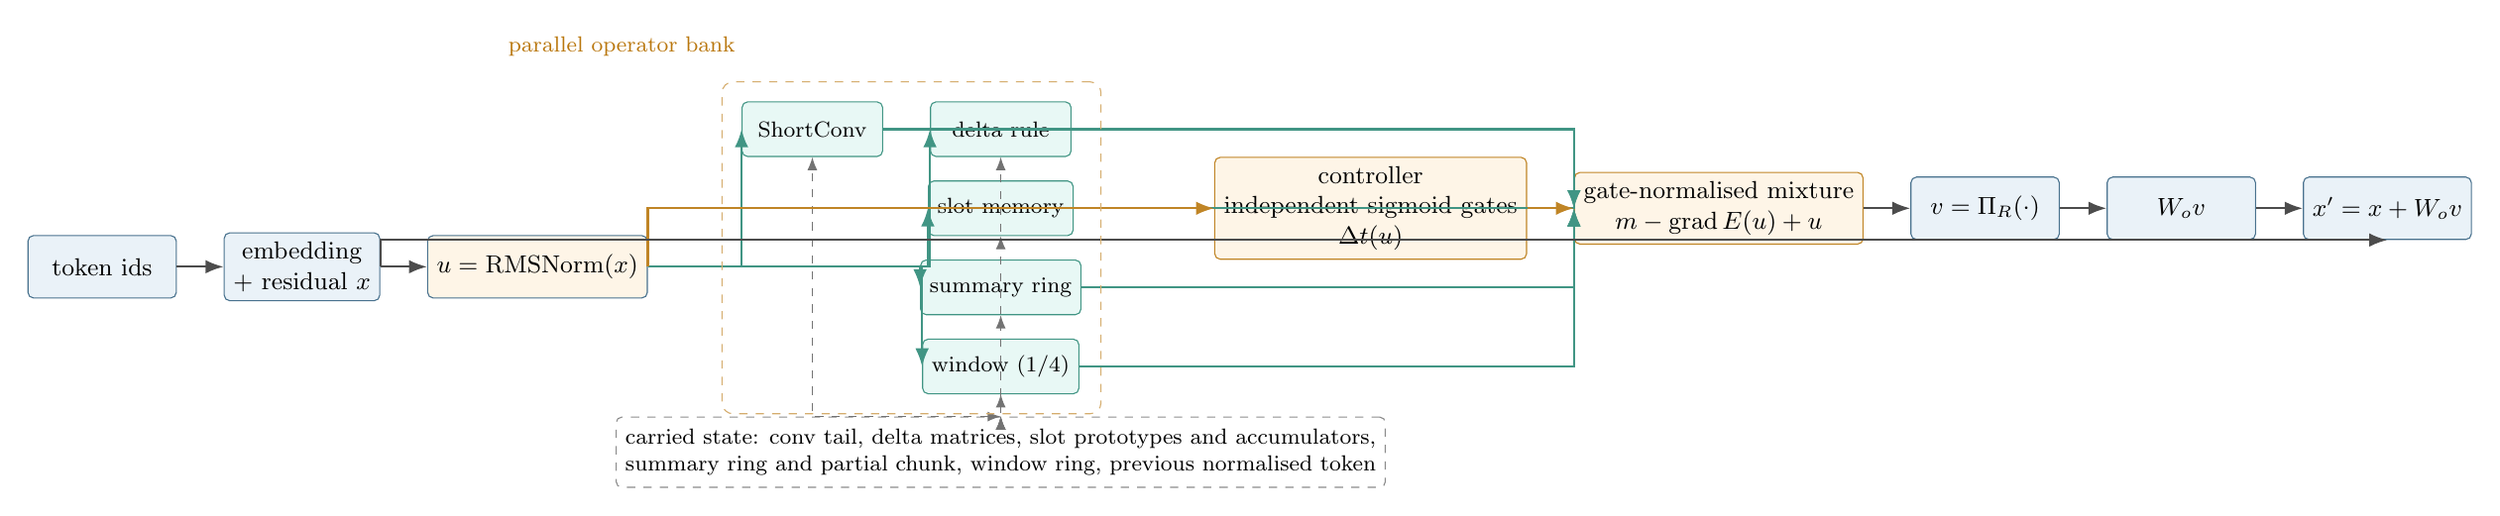
\begin{tikzpicture}[
  font=\small, >=Latex, node distance=4mm and 6mm,
  box/.style={draw=sigmaBlue!80, rounded corners=2pt, fill=lightBlue, align=center,
              minimum height=8mm, minimum width=19mm},
  op/.style={draw=sigmaTeal!80, rounded corners=2pt, fill=lightTeal, align=center,
             minimum height=7mm, minimum width=18mm, font=\footnotesize},
  ctrl/.style={draw=sigmaOrange!90, rounded corners=2pt, fill=lightOrange, align=center,
               minimum height=8mm, minimum width=24mm},
  state/.style={draw=black!45, dashed, rounded corners=2pt, fill=white, align=center,
                minimum height=9mm, minimum width=32mm, font=\footnotesize},
  arrow/.style={->, thick, draw=black!70},
  darrow/.style={->, thick, draw=sigmaTeal!80},
  carrow/.style={->, thick, draw=sigmaOrange!90},
  statearrow/.style={<->, dashed, draw=black!55}
]
\node[box] (tok) {token ids};
\node[box, right=of tok] (embed) {embedding\\+ residual $x$};
\node[box, right=of embed, fill=lightOrange] (norm) {$u=\rms(x)$};
\node[op, above right=10mm and 12mm of norm] (conv) {ShortConv};
\node[op, right=of conv] (delta) {delta rule};
\node[op, below=3mm of delta] (slot) {slot memory};
\node[op, below=3mm of slot] (summ) {summary ring};
\node[op, below=3mm of summ] (win) {window (1/4)};
\node[ctrl, right=18mm of slot] (ctrl) {controller\\independent sigmoid gates\\$\Delta t(u)$};
\node[ctrl, right=of ctrl] (mix) {gate-normalised mixture\\$m-\mathrm{grad}\,E(u)+u$};
\node[box, right=of mix] (proj) {$v=\Proj(\cdot)$};
\node[box, right=of proj] (out) {$W_o v$};
\node[box, right=of out] (add) {$x'=x+W_o v$};
\node[state, below=13mm of summ] (state) {carried state: conv tail, delta matrices, slot prototypes and accumulators,\\
summary ring and partial chunk, window ring, previous normalised token};

\draw[arrow] (tok) -- (embed);
\draw[arrow] (embed) -- (norm);
\foreach \op in {conv,delta,slot,summ,win} {
  \draw[darrow] (norm.east) -| (\op.west);
  \draw[darrow] (\op.east) -| (mix.west);
  \draw[statearrow] (state.north) -| (\op.south);
}
\draw[carrow] (norm.east) |- (ctrl.west);
\draw[carrow] (ctrl) -- (mix);
\draw[arrow] (mix) -- (proj);
\draw[arrow] (proj) -- (out);
\draw[arrow] (out) -- (add);
\draw[arrow] (embed.east) |- (add.south);

\node[draw=sigmaOrange!60, dashed, rounded corners, fit=(conv)(delta)(slot)(summ)(win), inner sep=2.5mm,
      label={[sigmaOrange, font=\footnotesize, yshift=2mm]above left:parallel operator bank}] {};
\end{tikzpicture}}
\caption{Implemented SigmaStorm dataflow. The normalised latent $u$ is sent to the enabled
operators in parallel; each operator reads and updates only its own carried state. The controller
produces independent gates and the step size, the gate-normalised mixture is combined with the
energy gradient and latent residual, and the projected proposal is added to the residual stream.
The diagram is a dataflow contract, not a literal tensor-layout drawing.}
\label{fig:architecture}
\end{figure*}

\subsection{The block}

A sequence is processed as a stream. For each token position $t$ the model keeps a residual
stream $x_t\in\R^{d}$ and a fixed-size recurrent state $S_t$. One block applies
\Cref{eq:block} once: normalise, offer the normalised latent to the enabled operators, mix
their proposals, subtract an energy gradient, and project. Stacking $L$ blocks applies the law
$L$ times to the token-local latent, while $S_t$ carries information across tokens.

Three details are not cosmetic.
\begin{itemize}[leftmargin=1.1em]
\item \textbf{Independent sigmoid gates.} A softmax over operators forces them to compete for
      a fixed total and can suppress an operator that is useful on a particular token. Independent
      sigmoids let any subset contribute simultaneously; they are mixture weights, not a compute
      skipping mechanism.
\item \textbf{Convex normalisation.} Dividing by the gate sum keeps the proposal scale from
      growing merely because more operators are enabled. The normalisation is a stability device,
      not evidence that any particular routing distribution is optimal.
\item \textbf{Per-operator RMSNorm.} Normalising each proposal before gating puts heterogeneous
      operator outputs on a comparable scale, so the gate is not dominated by an arbitrary raw
      output magnitude.
\end{itemize}

The step size is $\Delta t(u)=\Delta t\,(0.5+\sigma(a^\top u))$ with $\Delta t=0.5$ by default.
The projection acts on the latent $v$ only, never on the residual stream; this is what keeps
token identity available to the associative operator.

\subsection{Operator family}

\Cref{tab:operators} lists the operators, their role, intended fixed-configuration cost, and
state size. Window attention is enabled on one block in four by default and can be removed
entirely; it retains a bounded ring history. The current implementation also materialises a mask
over each input chunk, so the strict bounded-window runtime expression below should not be read as
a guarantee for arbitrarily large unchunked calls.

\begin{table*}[t]
\centering
\caption{Operators in the SigmaStorm block. Costs are per sequence of length $T$; state is
per sample and independent of $T$. $k$ is the convolution kernel, $H$ the number of delta
heads, $k_{\mathrm{exp}}$ the state-expansion factor, $d_h=d/H$ the head width, $S$ the number
of summary slots, and $W$ the window length.}
\label{tab:operators}
\small
\begin{tabularx}{\textwidth}{@{}l X l l@{}}
\toprule
Operator & Role & Cost & State \\
\midrule
ShortConv & local order; the fast proposal & $O(Tkd)$ & $k-1$ tokens \\
Gated delta rule & associative recall (key$\to$value bindings) & linear in $T$ for fixed chunks and width & $H k_{\mathrm{exp}}$ matrices $d_h\times d_h$ \\
Slot memory & long-horizon prototypes with per-token gated writes & $O(T n_s d)$ & $n_s\times d$ + accumulators \\
Chunk summaries & bounded global summary path without $T^2$ & $O(TSd)$ & ring of $S$ summaries \\
Window attention & precise local copying (1 block in 4, optional) & bounded-window intent; chunk-mask caveat above & ring buffer $W\times d$ \\
Energy potential & contraction and stabiliser, $-\nabla E$ & $O(Td r)$ for rank $r$ & none \\
Bounded projection & hard norm bound $\|v\|\leq R$ & $O(Td)$ & none \\
Gated FFN / MoE & per-token compute & $O(Td\,d_{\mathrm{ff}})$ & none \\
\bottomrule
\end{tabularx}
\end{table*}

\subsection{Energy contraction}
\label{sec:method-energy}

The potential is
\begin{equation}
  \begin{aligned}
  E(u)&=\tfrac12 u^\top D u+\tfrac12\|L^\top u\|^2,\\
  -\nabla E(u)&=-(Du+LL^\top u),
  \end{aligned}
\end{equation}
with $D$ diagonal positive and $L\in\R^{d\times r}$ low-rank. $E$ is strongly convex, so
$-\nabla E$ is an anisotropic contraction towards the origin. It is a stabiliser, not a
multi-basin memory: strong convexity forbids many equilibria by construction. The slot memory
and the delta rule are what hold information; the energy term keeps the latent from drifting
and makes the projected dynamics well behaved. An earlier design that treated the latent as a
multi-well attractor produced no usable memory and was discarded.

\subsection{Bounded projection}

The projection is $\Proj(z)=z\cdot\min(1,R/\|z\|)$ with $R=16$. It is applied after the
transition and before the output projection. Because the residual stream is additive
($x'=x+W_ov$), the bound constrains the \emph{proposal}, not the accumulated representation;
this distinction was one of the three fixes that took MQAR from chance to $0.97$.

\subsection{State contract and chunk invariance}

\begin{observation}[Carried-state chunking contract]
\label{obs:chunk}
For a fixed configuration, carrying the state $S_t$ of \Cref{tab:state} between contiguous
chunks is intended to make the hidden representation independent of the caller's chunk
boundaries. The current gate tests one split at position 50, inside both a 64-token slot block
and a 32-token summary block; it reports a maximum hidden-state difference of
$1.6\times10^{-6}$. This is an implementation check for that configuration, not an empirical
claim over every possible boundary, length, or hardware backend.
\end{observation}

\paragraph{Why the contract is plausible.}
Every operator in \Cref{tab:operators} is implemented as a causal scan whose value at position
$t$ depends on its carried state and tokens up to $t$. The short convolution carries its $k-1$
token tail; the delta rule carries its matrices and end-of-chunk state; the slot memory carries
the ring of prototypes \emph{and} unconsolidated write accumulators; the summary ring carries
completed summaries and its partial-chunk accumulator; and the window carries its ring buffer
and length. The controller and energy are token-local. These are the design conditions needed
for boundary independence. Gradient detaching changes the backward graph, not the forward
state update.

\begin{table}[t]
\centering
\caption{Carried state per block. No field has a dimension that grows with the processed length
$T$ for a fixed configuration. The slot and summary accumulators preserve partial work across
caller chunks; the reported equivalence result is limited to the tested configuration.}
\label{tab:state}
\small
\begin{tabular}{@{}l l@{}}
\toprule
Field & Shape / content \\
\midrule
\texttt{conv\_tail} & $[B,k-1,d]$ \\
\texttt{ssm} & $[B,Hk_{\mathrm{exp}},d_h,d_h]$ \\
\texttt{memory} & keys, values, usage, write accumulators \\
\texttt{summary} & $[B,H,S,d_h]^{\times 2}$ + usage/pos + partial chunk \\
\texttt{window} & $[B,H,W,d_h]^{\times 2}$ \\
\texttt{win\_len} & scalar \\
\texttt{prev} & $[B,d]$ (previous normalised token) \\
\bottomrule
\end{tabular}
\end{table}

\subsection{Streaming forward and update lifecycle}
\label{sec:algorithm}

\begin{figure*}[t]
\centering
\fbox{\begin{minipage}{0.94\textwidth}
\textbf{Algorithm 1: carried-state training step.}
\begin{enumerate}[leftmargin=1.6em]
\item Initialise the block states once at the beginning of a sequence. Do not reset them at a
      caller-defined micro-chunk boundary.
\item For each micro-chunk, run every block from the incoming state. Within a block, compute
      $u=\rms(x)$, evaluate the enabled operators from $u$ and their carried states, form the
      gate-normalised mixture, apply the energy step and bounded projection, then add the
      projected proposal to the residual stream. Return the updated state with the chunk output.
\item Accumulate language-model and configured multi-token-prediction losses from flat token
      slices. Repeat for \texttt{bptt\_chunks} micro-chunks while carrying the forward state.
\item Detach the carried state at the truncated-backpropagation boundary, backpropagate the
      accumulated loss, unscale and clip gradients when using mixed precision, then perform the
      optimiser update and clear the accumulation window.
\item Save checkpoints at the configured cadence, including the architecture configuration and
      optimiser state needed to resume. Evaluation and generation carry state across chunks but
      do not perform optimiser updates.
\end{enumerate}
\end{minipage}}
\caption{The implemented streaming lifecycle. State detachment limits gradient history; it does
not reset the forward memory. The algorithm describes the current training/evaluation interface,
not an instruction-tuning or preference-optimisation pipeline.}
\label{fig:stream-algorithm}
\end{figure*}

\subsection{Training interface}

Training processes \texttt{micro\_chunk} tokens per forward call (default 512 in the current
training interface) and carries the state within a sequence. The differentiable horizon is
$\texttt{bptt\_chunks}\times\texttt{micro\_chunk}$ (default $4\times512=2048$ tokens); the
state is detached at the window boundary. One reported Kaggle training profile used
256-token micro-chunks, so the paper reports the configured value rather than treating one
profile as a universal default. Forward context is not limited by this horizon, but gradients
are. Distributed execution uses DDP with \texttt{no\_sync} on all but the final backward and
an fp16/bf16 scaler protocol of unscale--clip--step--update. The schedule is warmup--stable--decay;
multi-token-prediction heads are ramped from zero; the sequence length can be ramped from short
windows to long ones. Cross-entropy is computed over flat token slices, never as a
$[B,T,\text{vocab}]$ tensor. Full hyperparameters are in \Cref{app:configs}; the defaults are
interface defaults, not a claim that every reported run used them.

\subsection{Implementation invariants}

Five implementation invariants were found while bringing the stack from chance-level to working
recall. They are documented because violating any one can silently damage the result:
\begin{enumerate}[leftmargin=1.2em]
\item \textbf{The delta-rule key is the previous token.} A binding is written when the value
      arrives at $t$; its key is the token at $t-1$. Reading query, key, and value all from
      $t$ forces the projections to disentangle a blended pair, and they do not.
\item \textbf{The delta rule reads the clean stream, and the decay bias is protected from the
      generic initialiser.} A generic ``initialise every bias to zero'' pass resets
      $\alpha=\exp(-\mathrm{softplus}(\cdot))$ to $0.5$ per token, and bindings vanish in two
      steps.
\item \textbf{The transition is an additive residual with a convex mixture.} Replacing the
      residual stream with the raw latent saturates the bound and erases token identity.
\item \textbf{Operator scale is controlled before mixing.} Per-operator RMSNorm and
      gate-sum normalisation keep the mixture from being dominated by raw output scale or by
      the number of open gates; this is a stability condition, not a measured quality gain.
\item \textbf{MQAR keys must be unique per sequence.} Sampling with replacement creates
      ambiguous queries and caps the achievable score near $0.6$.
\end{enumerate}

\section{Structured memory operators}
\label{sec:memory}

\subsection{The delta rule: associative recall}
\label{sec:delta}

Per head, with $a_t=\exp(g_t)$ and $b_t=\sigma(\beta_t)$,
\begin{equation}
\label{eq:delta-seq}
S_t=a_t S_{t-1}+b_t\,k_t\big(v_t-a_t k_t^\top S_{t-1}\big)^\top,
\qquad o_t=q_t^\top S_t .
\end{equation}
The term $(v_t-a_t k_t^\top S_{t-1})$ is error correction: the state is rewritten only by the
part of the value it does not already predict. This is what makes a repeated key overwrite its
binding instead of averaging all values ever seen with that key.

For training, the recurrence is evaluated in chunks of 64 tokens:
\begin{align}
A[i,j]&=\exp(g_i-g_j)\,b_j\,(k_i\!\cdot\!k_j), \quad j<i,\\
r&=(I+A)^{-1}\big(V-\exp(g)\odot K S_0\big),\\
O&=\exp(g)\odot Q S_0+\operatorname{tril}\!\big(\exp(g_i-g_j)b_j(q_i\!\cdot\!k_j)\big)\,r,\\
S_C&=\exp(g_{\mathrm{last}})S_0+\big(\exp(g_{\mathrm{last}}-g_j)b_jK\big)^\top r .
\end{align}
Every ratio on the causal region is at most one, so the chunkwise form cannot overflow. A
falsification gate compares it to the token-by-token reference and measures a maximum output
difference of $4.17\times10^{-7}$ (\Cref{tab:gates}).

\subsubsection{Decay spectrum (Gap A)}
\label{sec:gap-a-method}
A single decay rate gives the model one timescale: it must either forget local context quickly
or forget long-range bindings slowly, and it cannot do both. Each head therefore starts at its
own log-spaced rate,
\begin{equation}
\label{eq:spectrum}
\begin{aligned}
\mathrm{rate}_h&=r_{\min}\Big(\frac{r_{\max}}{r_{\min}}\Big)^{h/(H-1)},\\
\mathrm{bias}_h&=\log\!\big(\exp(\mathrm{rate}_h)-1\big),
\end{aligned}
\end{equation}
with $r_{\min}=10^{-4}$ and $r_{\max}=3\times10^{-2}$, i.e.\ $\alpha\approx0.9999$ down to
$0.970$. The projection weight is zero at initialisation, so these are exactly the initial
rates, and every rate remains a learned, token-dependent function. The initialiser protects the
bias from the generic zero-initialisation pass (invariant 2 in \Cref{sec:method}). The result
is a multiscale memory at step zero: some heads can hold a binding for the whole sequence,
others track the last few dozen tokens.

\subsection{State expansion (Gap B)}
\label{sec:gap-b-method}
\texttt{state\_expand}$=k$ multiplies the number of independent delta states without shrinking
each head:
\begin{equation}
\begin{aligned}
q,k,v&: d\to k\,d,\\
S&:[Hk,\,d_h,\,d_h],\qquad \text{output}: k\,d\to d,
\end{aligned}
\end{equation}
with $d_h=d/H$. Capacity and cost grow linearly, and unlike widening $d_h$ this does not reduce
the number of retrieval directions per token. The decay spectrum is laid out over all $Hk$
heads, so the extra states also add timescales. The \emph{capacity} benefit is not demonstrated
at the scale tested (\Cref{sec:results-gap-bc}); the mechanism is implemented and the state
remains constant in $T$.

\subsection{Slot memory: gated writes and a gated read (Gap D)}
\label{sec:slot}

A fixed ring of prototypes $K_j,V_j$ ($j=1\ldots n_s$) is updated per token. Routing is a
load-balanced soft assignment,
\begin{equation}
\label{eq:route}
a_{tj}=\softmax_j\!\Big(\frac{k_t\!\cdot\!K_j-\lambda\log(1+W_j)}{\tau_w}\Big),
\end{equation}
where $W_j$ is the causal write mass in the current block and $\lambda=1$ penalises routing
into an already-loaded slot. Without the penalty, sharp routing sends every similar token to
the same slot and the ring collapses to one prototype.

\paragraph{Write gate.}
Both novelty and evidence gate the write:
\begin{equation}
\label{eq:write-gate}
g_t=\Big[\frac{\nu_t-\delta}{1-\delta}\Big]_{+}\,e_t,
\qquad
\nu_t=1-\max_j\cos(k_t,K_j),
\end{equation}
where $\delta$ is the novelty floor and $[\cdot]_+=\max(\cdot,0)$. Novelty is computed twice:
first against the consolidated prototypes, then causally against writes earlier in the same
block. The second pass suppresses a repeated filler on its second occurrence instead of
flooding the accumulator. The floor is a dead-zone, not a damping heuristic: below $\delta$ the
write weight is exactly zero, so a repeated token cannot leak into every slot. Above the floor,
the novelty term is linearly rescaled by the fixed factor $1-\delta$ before multiplication by
the evidence gate; the resulting gradient is not literally unchanged.

\paragraph{Consolidation.}
Writes accumulate for \texttt{slot\_block} tokens and are consolidated with a Bayesian weight
\begin{equation}
\label{eq:consolidate}
D_j=\sum_t g_t a_{tj},\quad \eta_j=\frac{D_j}{D_j+1},
\end{equation}
\begin{equation}
\begin{aligned}
V_j&\leftarrow(1-\eta_j)V_j+\eta_j\frac{\sum_t g_t a_{tj}v_t}{D_j},\\
K_j&\leftarrow\mathrm{normalize}\!\Big((1-\eta_j)K_j\\
&\qquad+\eta_j\,\mathrm{normalize}\big(\textstyle\sum_t g_ta_{tj}k_t/D_j\big)\Big),\\
u_j&\leftarrow(1-\eta_j)u_j+\eta_j .
\end{aligned}
\end{equation}
One confident token moves a slot slightly; a block of agreeing tokens replaces it. The
accumulator, token counter, and ring are carried in the state, which is the mechanism's
chunking contract. The current equivalence gate tests this behavior at a split inside a slot
block; it does not measure every boundary, length, or backend.

\paragraph{Read gate.}
A softmax always hands out unit mass, so a query that matches nothing still receives a
full-scale average of every slot. The first version of this operator was therefore diffuse:
in a trained checkpoint the per-block read entropy was $3.03$--$3.16$ nats against
$\ln 24=3.178$, and zeroing the memory cost only $+0.035$ nats. Three changes turn the read
into a gated address:
\begin{equation}
\label{eq:read}
\begin{aligned}
m_t&=\max_{j:\,u_j>10^{-3}}\cos(q_t,K_j),\\
c_t&=\sigma\!\big(\kappa\,(m_t-\theta)\big),\\
\mathrm{read}_t&=c_t\,W_o\sum_j\softmax_j\!\big(s_{tj}/\tau_r\big)V_j,
\end{aligned}
\end{equation}
where $s_{tj}=q_t\!\cdot\!K_j$ is computed \emph{before} the usage bias, and $\kappa,\theta$ are
learned scalars. The separate read temperature $\tau_r$ is not the routing temperature: a read
that is sharp before addresses are trained picks an arbitrary slot. The confidence factor is a
differentiable abstention path: unmatched queries contribute zero and the residual stream alone
answers them. \Cref{fig:slot} shows the two paths. All three changes are opt-in
(\texttt{memory\_novelty\_floor}, \texttt{memory\_read\_temperature},
\texttt{memory\_abstain}); the defaults preserve the previous behaviour. Checkpoint
compatibility is governed by the saved architecture configuration and should be verified for
each artifact; this paper does not claim that arbitrary historical checkpoints accept every
future configuration.

\begin{figure*}[t]
\centering
\resizebox{\textwidth}{!}{%
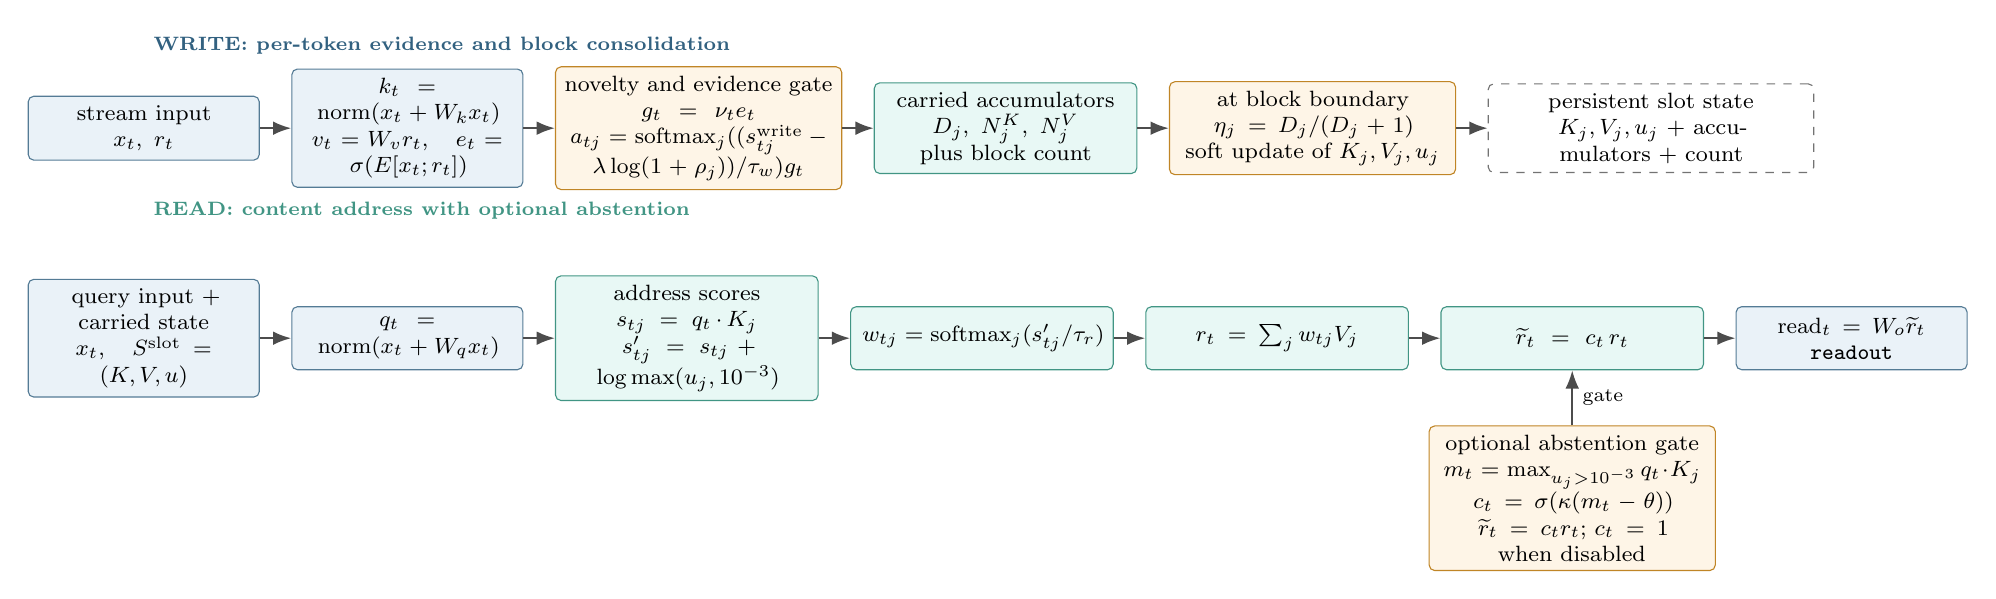
\begin{tikzpicture}[
  font=\footnotesize, >=Latex, node distance=3.5mm and 4mm,
  b/.style={draw=sigmaBlue!75, rounded corners=2pt, fill=lightBlue, align=center,
            minimum height=8mm, text width=27mm},
  g/.style={draw=sigmaOrange!90, rounded corners=2pt, fill=lightOrange, align=center,
            minimum height=8mm, text width=34mm},
  m/.style={draw=sigmaTeal!80, rounded corners=2pt, fill=lightTeal, align=center,
            minimum height=8mm, text width=31mm},
  state/.style={draw=black!55, dashed, rounded corners=2pt, fill=white, align=center,
                minimum height=9mm, text width=39mm},
  a/.style={->, thick, draw=black!70}
]

\node[anchor=west, font=\bfseries\scriptsize, text=sigmaBlue!90] at (0,1.05)
  {WRITE: per-token evidence and block consolidation};
\node[b] (winput) {stream input\\$x_t,\ r_t$};
\node[b, right=of winput] (features)
  {$k_t=\operatorname{norm}(x_t+W_kx_t)$\\
   $v_t=W_vr_t,\quad e_t=\sigma(E[x_t;r_t])$};
\node[g, right=of features] (routing)
  {novelty and evidence gate\\
   $g_t=\nu_te_t$\\
   $a_{tj}=\softmax_j((s^{\rm write}_{tj}
   -\lambda\log(1+\rho_j))/\tau_w)g_t$};
\node[m, right=of routing] (acc)
  {carried accumulators\\
   $D_j,\ N^K_j,\ N^V_j$\\
   plus block count};
\node[g, right=of acc] (consolidate)
  {at block boundary\\
   $\eta_j=D_j/(D_j+1)$\\
   soft update of $K_j,V_j,u_j$};
\node[state, right=of consolidate] (wstate)
  {persistent slot state\\
   $K_j,V_j,u_j$ + accumulators + count};

\draw[a] (winput) -- (features);
\draw[a] (features) -- (routing);
\draw[a] (routing) -- (acc);
\draw[a] (acc) -- (consolidate);
\draw[a] (consolidate) -- (wstate);

\node[anchor=west, font=\bfseries\scriptsize, text=sigmaTeal!80] at (0,-1.05)
  {READ: content address with optional abstention};
\node[b, below=15mm of winput] (rinput)
  {query input + carried state\\$x_t,\quad S^{\rm slot}=(K,V,u)$};
\node[b, right=of rinput] (query)
  {$q_t=\operatorname{norm}(x_t+W_qx_t)$};
\node[m, right=of query] (rawscore)
  {address scores\\
   $s_{tj}=q_t\!\cdot\!K_j$\\
   $s'_{tj}=s_{tj}+\log\max(u_j,10^{-3})$};
\node[m, right=of rawscore] (weights)
  {$w_{tj}=\softmax_j(s'_{tj}/\tau_r)$};
\node[m, right=of weights] (content)
  {$r_t=\sum_jw_{tj}V_j$};
\node[m, right=of content] (gated)
  {$\widetilde r_t=c_t\,r_t$};
\node[b, right=of gated] (output)
  {$\operatorname{read}_t=W_o\widetilde r_t$\\
   \texttt{readout}};
\node[g, below=7mm of gated] (confidence)
  {optional abstention gate\\
   $m_t=\max_{u_j>10^{-3}}q_t\!\cdot\!K_j$\\
   $c_t=\sigma(\kappa(m_t-\theta))$\\
   $\widetilde r_t=c_t r_t$; $c_t=1$ when disabled};

\draw[a] (rinput) -- (query);
\draw[a] (query) -- (rawscore);
\draw[a] (rawscore) -- (weights);
\draw[a] (weights) -- (content);
\draw[a] (content) -- (gated);
\draw[a] (gated) -- (output);
\draw[a] (confidence.north) -- node[right, font=\scriptsize] {gate} (gated.south);
\end{tikzpicture}}
\caption{Slot memory implementation, separated into its two causal paths. The write path forms
per-token keys, values, and evidence, computes novelty-aware assignments, accumulates them across
a fixed block, and then performs the soft consolidation update. The read path uses the carried
keys, values, and usage: the usage bias is added before the read softmax, while the optional
match-confidence gate is computed from the raw address score and applied to the value mixture
before the linear readout (equivalent to the displayed scalar form).
Dashed outlines mark state that is carried across calls; the figure does not draw a shortcut from
a write into the same token's read.}
\label{fig:slot}
\end{figure*}

\subsection{Chunk summaries: a bounded global path without $T^2$ (Gap C)}
\label{sec:summary}

Every \texttt{summary\_chunk} tokens, one pooled summary is written to a fixed ring of
\texttt{summary\_slots}:
\begin{equation}
\label{eq:summary}
\begin{aligned}
p_c&=\frac1C\sum_{t\in c}u_t,\qquad u_t=\rms(x_t),\\
q_t&=\mathrm{normalize}(W_qu_t),\\
K_c&=\mathrm{normalize}(W_kp_c),\qquad V_c=W_vp_c,\\
\mathrm{score}_{tc}&=q_t\!\cdot\!K_c/\sqrt{d_h}\\
&\qquad-\mathrm{softplus}(\gamma)\,(t_c^{\mathrm{idx}}-\mathrm{pos}_c),\\
o_t&=W_o\sum_c\softmax_c(\mathrm{score}_{tc})\,V_c .
\end{aligned}
\end{equation}
Cost is $O(TS\,d)$ for fixed summary count, width, and chunking, and state is constant in $T$.
The age bias is learned per head, so a summary can stay addressable for the retained ring or
fade. Only completed chunks are written; the partial-chunk accumulator is carried in the state.
This is a bounded global-summary path, not exact token-level retrieval for an unbounded sequence,
and it avoids constructing a $T\times T$ summary attention matrix. Its measured benefit is
discussed honestly in \Cref{sec:results-gap-bc}.

\section{Experimental methodology}
\label{sec:experiments}

\paragraph{Artifacts.}
All numerical results in this report are produced by scripts in the repository:
\texttt{scripts/gate.py} (falsification gates), \texttt{pytest tests} (unit tests),
\texttt{scripts/ladder.py} (controlled operator comparisons), \texttt{scripts/gapd\_proof.py}
(three-arm slot-read experiment), and the training/evaluation scripts for the 21M model.
Raw outputs are \texttt{results/ladder.\{json,md\}},
\texttt{results/gapd\_proof.\{json,md\}}, and \texttt{results/20m\_tinystories.md}.

\paragraph{Why synthetic tasks first.}
A language-model loss aggregates many capabilities and hides which operator failed. We
therefore isolate one capability per task before training a language model:
MQAR for delta-rule association, delayed recall by distance for the decay spectrum, a count
task for the summary path, and a frozen-embedding presence task for the slot memory. The
frozen-embedding detail matters: with a single supervised token per sequence, a trainable head
and tied embeddings can solve the task by collapsing token embeddings without using memory.
Freezing embeddings and untying the head removes that shortcut.

\paragraph{Tasks.}
\begin{itemize}[leftmargin=1.1em]
\item \textbf{MQAR.} Sequences contain key$\to$value bindings followed by queries; keys are
      unique per sequence. Accuracy is measured only on query answers. Chance is $1/n_{\mathrm{values}}$.
      The mechanism gate uses 32 keys and 16 values (chance $0.062$); the ladder baseline uses
      26 bindings and 16 values.
\item \textbf{Delayed recall.} Eight bindings are placed at controlled distances; the model is
      queried later. Accuracy is reported overall and in distance buckets $<32$, $32$--$127$,
      $128$--$255$, and $\geq256$ tokens.
\item \textbf{Aggregate recall.} Symbols are presented, then a count question is asked about a
      symbol seen roughly 150 tokens earlier ($\text{max count}=8$; chance $1/9$).
\item \textbf{Presence recall.} Sixteen symbols, eight present in the opening quarter of a
      192-token stream, filler afterwards, then a query token and a yes/no answer. Only the
      answer is supervised. Chance is $0.50$. The model is conv + slot memory only; token
      embeddings are frozen and the output head is untied.
\item \textbf{Language modeling.} TinyStories tokenised with an 8K byte-level BPE tokenizer,
      EOS between documents, a 300M training-token target and a 5M held-out-token target. The
      checked-in validation artifact contains 4{,}713{,}394 tokens, so the realized validation
      size is smaller than the build target. Held-out loss is measured on that split; perplexity
      is $\exp(\text{CE})$ within this tokenizer.
\end{itemize}

\paragraph{Protocol.}
Mechanism models use the \texttt{tiny} preset; task-specific overrides are listed in
\Cref{app:configs}. Unless stated otherwise: AdamW with learning rate $10^{-3}$, betas
$(0.9,0.95)$, weight decay $0.01$, gradient clipping at norm $1.0$. Batch sizes are 8--24
depending on the task; the presence experiment uses batch 8 and 800 steps, the aggregate
comparison 600 steps, and MQAR 400 steps. Seeds are reported individually because the
seed-to-seed spread is a first-class result, not a nuisance to be hidden by a mean. With two or
three seeds we do not compute significance tests; a difference smaller than the seed spread is
called inconclusive.

\paragraph{Metrics.}
Accuracy is the fraction of supervised answer tokens that are correct. Cross-entropy is
reported in nats per supervised token, $\mathrm{CE}=\text{lm\_sum}/\text{lm\_count}$, and
perplexity as $\exp(\mathrm{CE})$. Read entropy is
$H=-\sum_j p_j\log p_j$ averaged over tokens, with $\ln n_{\mathrm{slots}}$ the uniform
maximum. The memory ablation delta is
$\Delta_{\mathrm{abl}}=\mathrm{CE}(\text{memory output zeroed})-\mathrm{CE}(\text{normal})$;
a positive value means the memory is useful. State bytes are the sum of all carried tensors per
sample, measured at two context lengths to verify independence from $T$.

\paragraph{Hardware and honesty about it.}
The 21M language-model run used two 16\,GB T4 GPUs (fp16 DDP, 13.49\,GB peak per GPU). The
mechanism and Gap~D experiments in this report were re-run on CPU because the Kaggle weekly
GPU quota (30\,h) was exhausted; data, seeds, optimiser, and step counts are identical to the
GPU protocol. The forward-time measurements are single-machine CPU numbers with two threads and
should be read as relative cost, not deployment throughput.

\begin{table*}[t]
\centering
\caption{Claims and evidence map. ``Established'' means a controlled comparison or an
equivalence gate with a stated number; ``inconclusive'' means the observed difference is within
seed/task noise; ``not demonstrated'' means the mechanism exists but its benefit was not shown.
No row in this table is a frontier-scale claim.}
\label{tab:claims}
\small
\begin{tabularx}{\textwidth}{@{}l X l@{}}
\toprule
Claim & Evidence & Status \\
\midrule
Chunkwise delta rule equals the sequential rule & gate: max output diff $4.17\times10^{-7}$ & Established \\
Chunked forward equals full forward & gate: $1.6\times10^{-6}$, split inside slot/summary blocks & Established \\
State size is independent of context & 200{,}704 bytes at $T=512$ and $T=4096$ & Established \\
Decay spectrum improves long-range recall & $\geq256$: $1.000$ vs.\ $0.297$ (frozen rates) & Established (synthetic) \\
State expansion increases capacity & expand1 $0.754$ vs.\ expand2 $0.555$ at 66 bindings & Not demonstrated \\
Chunk summaries improve aggregate recall & $0.703$ with vs.\ $0.672$ without; an earlier $0.797$ vs.\ $0.891$ did not reproduce & Inconclusive \\
Gated slot read is content-addressed & presence $0.977/1.000/0.953$ vs.\ chance; $\Delta_{\mathrm{abl}}=+2.26$ nats & Established (synthetic) \\
Gated read leaves the checked controls close & MQAR is higher in both seeds; aggregate is mixed; one LM pair is $3.0826$ vs.\ $3.0760$ nats & Mixed; no improvement claim \\
Small language model trains and generates & 21M params, 348M tokens, held-out loss $1.2523$ / PPL $3.498$ & Prototype demonstrated \\
Competitive with transformers at LM & no matched LM baseline was trained & Not claimed \\
256K-token context works & no model trained at that context & Not demonstrated \\
\bottomrule
\end{tabularx}
\end{table*}

\section{Results}
\label{sec:results}

\subsection{Correctness gates}

\Cref{tab:gates} lists the falsification gates. They are not capability results; they establish
that the implementation matches its mathematical specification and that the state contract
holds. The chunked-forward gate is the important one for long context: the split point is
position 50, inside both a 64-token slot-consolidation block and a 32-token summary block, and
the chunked hidden state still matches the full forward to $1.6\times10^{-6}$.

\begin{table}[t]
\centering
\caption{Falsification gates (\texttt{scripts/gate.py}) and unit tests.}
\label{tab:gates}
\small
\begin{tabularx}{\columnwidth}{@{}>{\raggedright\arraybackslash}X r@{}}
\toprule
Gate & Measured \\
\midrule
Delta rule, chunkwise vs.\ sequential & $\max|\Delta o|=4.17\times10^{-7}$ \\
 & $\max|\Delta S|=3.58\times10^{-7}$ \\
Chunked vs.\ full forward (split at 50) & $\max|\Delta h|=1.55\times10^{-6}$ \\
State bytes at $T=512$ and $T=4096$ & $200{,}704$ (constant) \\
MQAR recall, 400 steps & $0.974$ vs.\ chance $0.062$ \\
Unit tests (\texttt{pytest tests}) & 21 passed \\
\bottomrule
\end{tabularx}
\end{table}

\subsection{Decay spectrum (Gap A)}
\label{sec:results-gap-a}

\Cref{tab:gap-a} and \Cref{fig:gap-a} report delayed recall at four distance buckets. The
comparison is deliberately isolated: the slot memory and summaries are disabled, and the decay
bias is frozen so the comparison measures the initialised prior. When the bias is trainable, a
single-rate model simply learns its own spectrum and the ablation shows nothing; that was the
first, invalid version of this experiment (\Cref{app:ledger}).

\begin{table}[t]
\centering
\caption{Delayed recall by distance (8 bindings, length 320, 300 steps). Frozen decay.}
\label{tab:gap-a}
\small
\begin{tabular}{@{}l c c c c c@{}}
\toprule
Variant & Overall & $<32$ & $32$--$127$ & $128$--$255$ & $\geq256$ \\
\midrule
full & 0.984 & 0.984 & 0.984 & 1.000 & 0.969 \\
spectrum & \textbf{1.000} & 1.000 & 1.000 & 1.000 & \textbf{1.000} \\
single rate & 0.758 & 0.984 & 1.000 & 0.750 & 0.297 \\
\bottomrule
\end{tabular}
\end{table}

\begin{figure}[t]
\centering
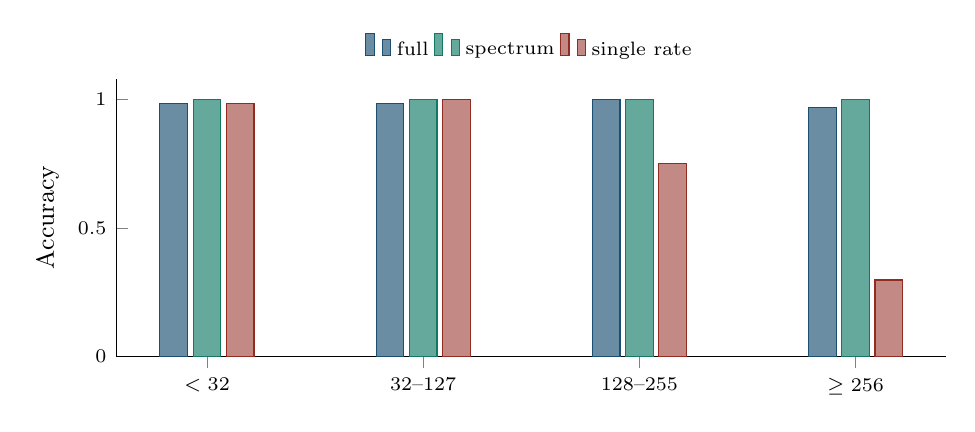
\begin{tikzpicture}
\begin{axis}[
  width=\columnwidth, height=5.1cm, ybar,
  ymin=0, ymax=1.08, ylabel={Accuracy}, ylabel style={font=\small},
  symbolic x coords={{$<32$},{$32$--$127$},{$128$--$255$},{$\geq256$}},
  xtick=data, x tick label style={font=\scriptsize}, y tick label style={font=\scriptsize},
  enlarge x limits=0.14,
  legend style={font=\scriptsize, draw=none, at={(0.5,1.03)}, anchor=south, legend columns=3},
  axis lines*=left
]
\addplot[fill=sigmaBlue!65, draw=sigmaBlue] coordinates
  {({$<32$},0.984) ({$32$--$127$},0.984) ({$128$--$255$},1.000) ({$\geq256$},0.969)};
\addplot[fill=sigmaTeal!65, draw=sigmaTeal] coordinates
  {({$<32$},1.000) ({$32$--$127$},1.000) ({$128$--$255$},1.000) ({$\geq256$},1.000)};
\addplot[fill=sigmaRed!55, draw=sigmaRed] coordinates
  {({$<32$},0.984) ({$32$--$127$},1.000) ({$128$--$255$},0.750) ({$\geq256$},0.297)};
\legend{full, spectrum, single rate}
\end{axis}
\end{tikzpicture}
\caption{Recall collapses with distance when all heads share one frozen decay rate. The
log-spaced spectrum holds every bucket; the full model is slightly below the delta-only
spectrum at the longest bucket because the comparison mixes additional operators.}
\label{fig:gap-a}
\end{figure}

The single rate is not broken at short distances: it reaches $0.984$ below 32 tokens and
$1.000$ at $32$--$127$. The failure is specifically long-range, $0.297$ beyond 256 tokens,
against $1.000$ for the spectrum. A single timescale cannot simultaneously forget local
context and preserve a binding across hundreds of tokens; the spectrum can.

\subsection{State expansion and chunk summaries (Gaps B and C)}
\label{sec:results-gap-bc}

\Cref{tab:gap-bc} reports the two comparisons whose benefit is \emph{not} established.

\begin{table}[t]
\centering
\caption{Gap B (dense MQAR, 66 bindings) and Gap C (aggregate count). Both tasks are
seed-noise-limited; see the text.}
\label{tab:gap-bc}
\small
\begin{tabularx}{\columnwidth}{@{}l r r@{}}
\toprule
Variant & Accuracy & Params \\
\midrule
\multicolumn{3}{@{}l}{\emph{Capacity: MQAR, 66 bindings (chance $0.125$)}}\\
\texttt{state\_expand}=1 & \textbf{0.754} & 1{,}694{,}911 \\
\texttt{state\_expand}=2 & 0.555 & 2{,}027{,}231 \\
\midrule
\multicolumn{3}{@{}l}{\emph{Aggregate count (chance $0.111$)}}\\
full (with summaries) & 0.703 & 2{,}080{,}744 \\
no summaries & 0.672 & 1{,}817{,}556 \\
\bottomrule
\end{tabularx}
\end{table}

\begin{figure}[t]
\centering
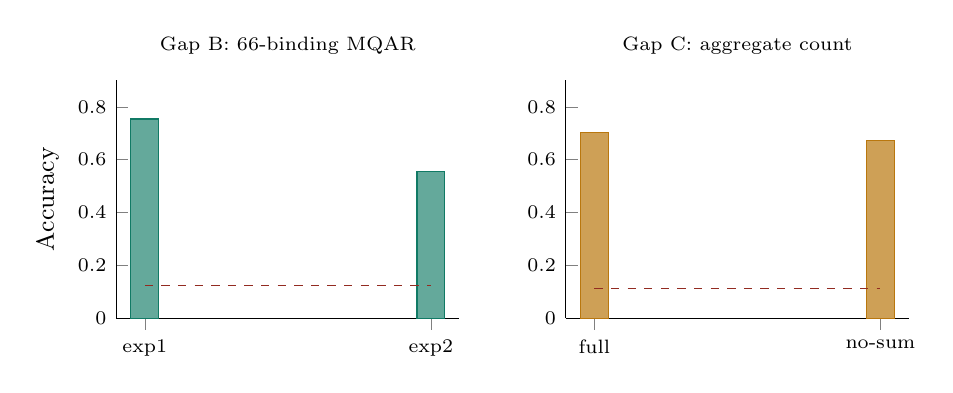
\begin{tikzpicture}
\begin{groupplot}[
  group style={group size=2 by 1, horizontal sep=1.35cm},
  width=0.49\columnwidth, height=4.6cm, ybar,
  ymin=0, ymax=0.9,
  tick label style={font=\scriptsize},
  ylabel style={font=\small}, x tick label style={font=\scriptsize},
  legend style={font=\scriptsize, draw=none},
  axis lines*=left
]
\nextgroupplot[title={\scriptsize Gap B: 66-binding MQAR}, ylabel={Accuracy},
  symbolic x coords={exp1,exp2}, xtick=data]
\addplot[fill=sigmaTeal!65, draw=sigmaTeal] coordinates {(exp1,0.754) (exp2,0.555)};
\draw[dashed, sigmaRed] (axis cs:exp1,0.125) -- (axis cs:exp2,0.125);
\nextgroupplot[title={\scriptsize Gap C: aggregate count},
  symbolic x coords={full,no-sum}, xtick=data]
\addplot[fill=sigmaOrange!70, draw=sigmaOrange] coordinates {(full,0.703) (no-sum,0.672)};
\draw[dashed, sigmaRed] (axis cs:full,0.111) -- (axis cs:no-sum,0.111);
\end{groupplot}
\end{tikzpicture}
\caption{Neither extra state capacity nor the summary ring shows a reliable benefit at the
tested budget. Dashed lines are chance. These are negative/inconclusive results, not hidden
failures.}
\label{fig:gap-bc}
\end{figure}

\textbf{State expansion.} Doubling the number of independent delta states did not improve
dense MQAR; it reduced accuracy from $0.754$ to $0.555$. The task has 66 bindings, above the
practical rank of one $32\times32$ state per head, so one might expect capacity to help. It
did not at 300 steps. Possible explanations are optimisation (the larger model needs more
steps) or interference between duplicated state matrices; the experiment does not distinguish
them. We therefore do not claim a capacity benefit.

\textbf{Chunk summaries.} The aggregate count task improves by $0.031$ with summaries,
$0.703$ vs.\ $0.672$. An earlier run measured $0.797$ with summaries and $0.891$ without,
\ie the opposite sign. The metric is noise-limited at this budget, and the summary change was
not adopted on the strength of either run. The operator is correct and chunk-invariant; its
quality benefit remains unproven.

\subsection{The gated slot read (Gap D)}
\label{sec:results-gap-d}

\Cref{tab:presence} reports the three-arm presence experiment: the previous cosine read, the
ZCA-whitened read on its own, and the shipped gated mechanism (novelty dead-zone, read
temperature, abstention). All arms use identical data, seeds, optimiser, and 800 steps.

\begin{table}[t]
\centering
\caption{Presence recall with frozen embeddings (16 symbols, 8 present, chance $0.50$).
Means over seeds are shown for readability; individual seeds are the evidence.}
\label{tab:presence}
\small
\begin{tabularx}{\columnwidth}{@{}l c c c c@{}}
\toprule
Arm & Seed 0 & Seed 1 & Seed 2 & Mean \\
\midrule
cosine (previous) & 0.562 & 0.539 & 0.555 & 0.552 \\
ZCA-whitened & 0.648 & 0.531 & 0.539 & 0.573 \\
\textbf{gated} & \textbf{0.977} & \textbf{1.000} & \textbf{0.953} & \textbf{0.977} \\
\bottomrule
\end{tabularx}
\end{table}

\begin{figure*}[t]
\centering
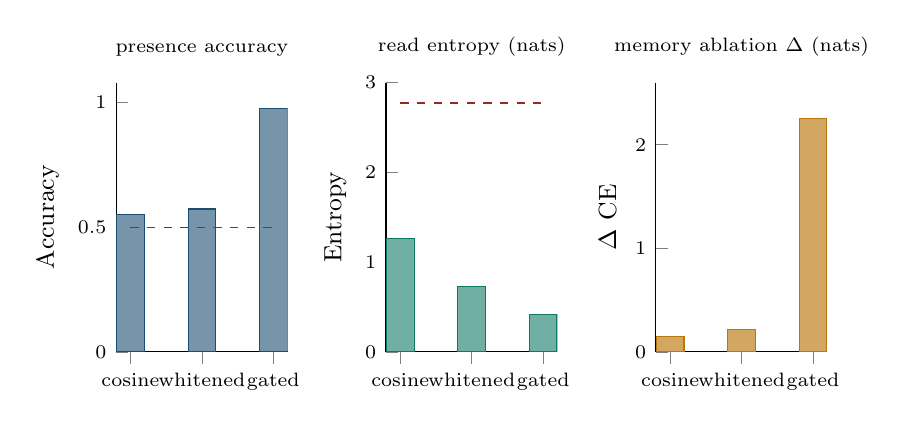
\begin{tikzpicture}
\begin{groupplot}[
  group style={group size=3 by 1, horizontal sep=1.25cm},
  width=0.31\textwidth, height=5.0cm, ybar,
  tick label style={font=\scriptsize}, ylabel style={font=\small},
  axis lines*=left, ymin=0
]
\nextgroupplot[title={\scriptsize presence accuracy}, ylabel={Accuracy}, ymax=1.08,
  symbolic x coords={cos,whiten,gated}, xtick=data,
  xticklabels={cosine,whitened,gated}]
\addplot[fill=sigmaBlue!60, draw=sigmaBlue] coordinates {(cos,0.552) (whiten,0.573) (gated,0.977)};
\draw[dashed, sigmaRed] (axis cs:cos,0.50) -- (axis cs:gated,0.50);
\nextgroupplot[title={\scriptsize read entropy (nats)}, ylabel={Entropy}, ymax=3.0,
  symbolic x coords={cos,whiten,gated}, xtick=data,
  xticklabels={cosine,whitened,gated}]
\addplot[fill=sigmaTeal!60, draw=sigmaTeal] coordinates {(cos,1.2595) (whiten,0.7246) (gated,0.4132)};
\draw[dashed, sigmaRed] (axis cs:cos,2.7726) -- (axis cs:gated,2.7726);
\nextgroupplot[title={\scriptsize memory ablation $\Delta$ (nats)}, ylabel={$\Delta$ CE}, ymax=2.6,
  symbolic x coords={cos,whiten,gated}, xtick=data,
  xticklabels={cosine,whitened,gated}]
\addplot[fill=sigmaOrange!65, draw=sigmaOrange] coordinates {(cos,0.1467) (whiten,0.2173) (gated,2.2551)};
\end{groupplot}
\end{tikzpicture}
\caption{Gap D in one view. Whitening sharpens the read (entropy falls) but does not make it
useful; the gated read both sharpens it and makes it load-bearing, as shown by the ablation
delta. Dashed lines: chance accuracy, uniform entropy $\ln16=2.773$ nats.}
\label{fig:gap-d}
\end{figure*}

\begin{table}[t]
\centering
\caption{Gap D diagnostics, seed 0, 16 slots. Uniform read entropy is $\ln16=2.773$ nats.}
\label{tab:gap-d-diag}
\small
\begin{tabularx}{\columnwidth}{@{}l c c c c c@{}}
\toprule
Arm & Entropy & Top $w$ & Key cos & CE & $\Delta_{\mathrm{abl}}$ \\
\midrule
cosine & 1.260 & 0.608 & 0.023 & 0.663 & $+0.147$ \\
whitened & 0.725 & 0.788 & $-0.044$ & 0.517 & $+0.217$ \\
gated & \textbf{0.413} & \textbf{0.820} & 0.004 & \textbf{0.019} & $\mathbf{+2.255}$ \\
\bottomrule
\end{tabularx}
\end{table}

The gated read is not merely sharper; it is discriminating. Match confidence averages
$0.562$ on present queries and $0.026$ on absent ones, \ie the abstention path separates the
two populations without supervision on the gate. The ablation delta shows the same from the
other side: zeroing the memory now costs $2.26$ nats, against $0.15$ before, so the residual
stream alone can no longer answer the task. ZCA whitening sharpens entropy from $1.26$ to
$0.72$ nats but leaves accuracy at chance, because it amplifies every deviation direction,
including context noise.

\paragraph{No-regression controls.}
The gated mechanism must not break the paths it does not target. \Cref{tab:regression} shows
MQAR (delta-rule path), aggregate recall (summary path), and a 600-step real-data next-token
comparison on the tiny preset. MQAR is unchanged to within seed noise, and is slightly higher
for the gated arm ($+0.002$ and $+0.008$). The aggregate task is seed-noisy but the gated arm
is above the previous behaviour on both seeds. Real-data language modeling moves val CE from
$3.0760$ to $3.0826$ nats, a $0.2\%$ difference inside the run-to-run spread; the training
curves overlap throughout (\Cref{fig:lm-check}).

\begin{table}[t]
\centering
\caption{No-regression controls for the gated read. MQAR: 400 steps, 2 seeds. Aggregate:
600 steps, 2 seeds. LM: tiny preset, 3.06M params, 600 steps, identical stream.}
\label{tab:regression}
\small
\begin{tabularx}{\columnwidth}{@{}l c c@{}}
\toprule
Measure & previous & gated \\
\midrule
MQAR seed 0 & 0.988 & \textbf{0.990} \\
MQAR seed 1 & 0.979 & \textbf{0.987} \\
Aggregate seed 0 & 0.680 & \textbf{0.836} \\
Aggregate seed 1 & 1.000 & 0.859 \\
LM val CE (nats) & \textbf{3.0760} & 3.0826 \\
LM PPL & 21.67 & 21.82 \\
\bottomrule
\end{tabularx}
\end{table}

\begin{figure}[t]
\centering
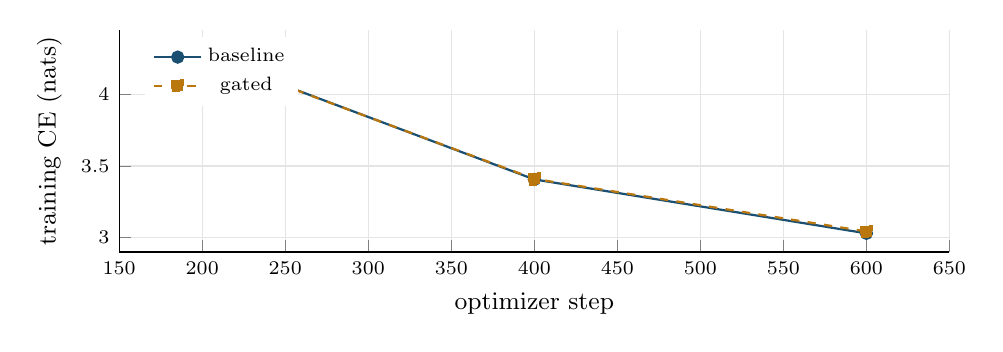
\begin{tikzpicture}
\begin{axis}[
  width=\columnwidth, height=4.4cm,
  xlabel={optimizer step}, ylabel={training CE (nats)},
  xmin=150, xmax=650, ymin=2.9, ymax=4.45,
  tick label style={font=\scriptsize}, label style={font=\small},
  legend style={font=\scriptsize, draw=none, at={(0.03,0.97)}, anchor=north west},
  axis lines*=left, grid=major, grid style={black!10}
]
\addplot[thick, sigmaBlue, mark=*] coordinates {(200,4.2786) (400,3.4066) (600,3.0300)};
\addplot[thick, sigmaOrange, mark=square*, dashed] coordinates {(200,4.2745) (400,3.4105) (600,3.0431)};
\legend{baseline, gated}
\end{axis}
\end{tikzpicture}
\caption{Real TinyStories next-token training, identical stream. The gated slot read does not
change the loss trajectory. Held-out CE is $3.0760$ (baseline) vs.\ $3.0826$ (gated).}
\label{fig:lm-check}
\end{figure}

\subsection{Language modeling at 21M parameters}
\label{sec:results-lm}

The largest model in this report has 20{,}996{,}090 parameters (6 blocks, width 320, 8 heads,
\texttt{state\_expand}=2, 24 slots, 32 summary slots, no MoE). It was trained on TinyStories
(8K byte-level BPE, 300M-token training split) for 10{,}604 steps in two resumed sessions on
two T4 GPUs, a total of roughly 348M tokens. \Cref{tab:20m} reports the two held-out
evaluations.

\begin{table}[t]
\centering
\caption{21M TinyStories run, 2\,$\times$\,T4, fp16 DDP. Held-out evaluation is 20 batches of
4\,$\,$ $\times$\,1024 tokens (81{,}840 supervised tokens). MQAR is far out of distribution
and is reported for completeness only.}
\label{tab:20m}
\small
\begin{tabular}{@{}l c c c@{}}
\toprule
Session & Steps & Held-out loss & PPL \\
\midrule
1 & 5{,}442 & 1.3225 & 3.753 \\
2 & 10{,}604 & \textbf{1.2523} & \textbf{3.498} \\
\bottomrule
\end{tabular}
\end{table}

The model writes grammatical, on-genre TinyStories prose from a prompt. The checkpoint
predates the gated slot read; its slot memory is the diffuse version audited in
\Cref{tab:slotaudit}, which is exactly the defect Gap D removes. The language model is useful
as a prototype, not as evidence of general language ability: TinyStories is a restricted
synthetic corpus, the tokenizer is 8K byte-level BPE, and no transformer was trained on the
same data for comparison.

\begin{table}[t]
\centering
\caption{Slot-memory audit of the 21M checkpoint (pre-fix). Uniform read entropy is
$\ln24=3.178$ nats. Zeroing the read costs only $+0.035$ nats: the memory acts as a slow
average. This table motivates the gated read.}
\label{tab:slotaudit}
\small
\begin{tabular}{@{}c c c c@{}}
\toprule
Block & Read entropy & Top weight & Cross-slot cos \\
\midrule
0 & 3.133 & 0.065 & 0.465 \\
1 & 3.109 & 0.073 & 0.525 \\
2 & 3.160 & 0.070 & 0.810 \\
3 & 3.159 & 0.055 & 0.715 \\
4 & 3.048 & 0.131 & 0.716 \\
5 & 3.095 & 0.078 & 0.483 \\
\bottomrule
\end{tabular}
\end{table}

\begin{table*}[t]
\centering
\caption{Representative samples from the step-10{,}604 checkpoint (temperature 0.7, top-$k$ 40),
truncated. These show local coherence, not long-horizon recall.}
\label{tab:samples}
\small
\begin{tabularx}{\textwidth}{@{}>{\raggedright\arraybackslash}X@{}}
\toprule
``Once upon a time, there was a little girl named Lily. She loved to play with her toys and
make them into different things. One day, she found a toy that was different from the others.
It was a big, shiny rock that had a pointy edge\ldots'' \\
``The little dog ran into the garden and saw the flowers. He was so happy and he couldn't wait
to show all his friends. But then, something bad happened. A big dog came running and scared
the little dog away\ldots'' \\
``Tom was very sad because he lost his toy. He looked everywhere for it, but it was nowhere to
be found. He started to cry because he missed his toy so much. His mother was worried and
asked him what was wrong\ldots'' \\
\bottomrule
\end{tabularx}
\end{table*}

\subsection{Cost and state}
\label{sec:results-cost}

\Cref{tab:cost} compares SigmaStorm with the size-matched-in-width transformer control from
the experiment ladder. The control matches width, depth, heads, and FFN multiplier, not total
parameter count: SigmaStorm's operators add parameters, so at the same width it has about
$2.3$--$3.0\times$ more parameters and, on CPU, is roughly $2$--$9\times$ slower per forward
pass. There is no compute-efficiency claim here. The architectural advantage that motivates the
design is memory: state is constant in context (\Cref{tab:gates}), while a transformer KV cache
grows linearly. That advantage only matters if long-context training works at scale, which is
not demonstrated in this report.

\begin{table}[t]
\centering
\caption{Forward cost at equal width (CPU, two threads, batch 1). The transformer control
matches width/depth, not parameter count.}
\label{tab:cost}
\small
\begin{tabular}{@{}l r r r r@{}}
\toprule
Config & $\Sigma$ params & $\Sigma$ s & T params & T s \\
\midrule
tiny $T{=}128$ & 2.08M & 0.031 & 0.68M & 0.0036 \\
tiny $T{=}512$ & 2.08M & 0.102 & 0.68M & 0.0147 \\
tiny $T{=}2048$ & 2.08M & 0.411 & 0.68M & 0.1404 \\
20M $T{=}128$ & 20.97M & 0.094 & 8.37M & 0.0180 \\
20M $T{=}512$ & 20.97M & 0.321 & 8.37M & 0.0761 \\
20M $T{=}2048$ & 20.97M & 1.339 & 8.37M & 0.5872 \\
\bottomrule
\end{tabular}
\end{table}

\begin{figure}[t]
\centering
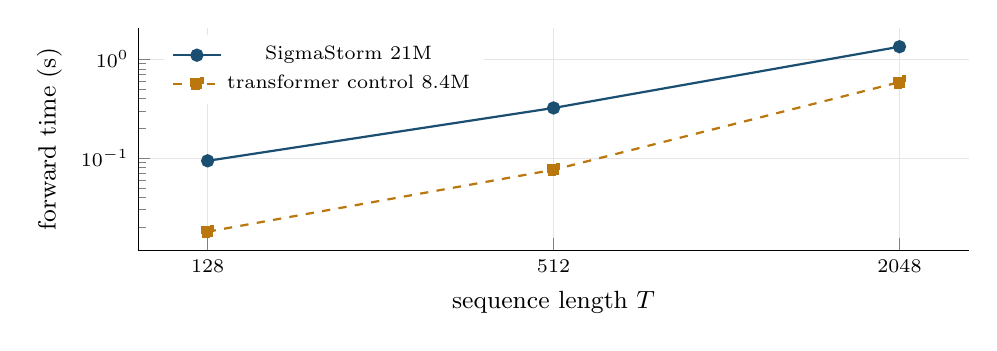
\begin{tikzpicture}
\begin{axis}[
  width=\columnwidth, height=4.4cm,
  xlabel={sequence length $T$}, ylabel={forward time (s)},
  xmode=log, ymode=log, log basis x=2,
  xtick={128,512,2048}, xticklabels={128,512,2048},
  tick label style={font=\scriptsize}, label style={font=\small},
  legend style={font=\scriptsize, draw=none, at={(0.03,0.97)}, anchor=north west},
  axis lines*=left, grid=major, grid style={black!10}
]
\addplot[thick, sigmaBlue, mark=*] coordinates {(128,0.0938) (512,0.3214) (2048,1.3388)};
\addplot[thick, sigmaOrange, mark=square*, dashed] coordinates {(128,0.0180) (512,0.0761) (2048,0.5872)};
\legend{SigmaStorm 21M, transformer control 8.4M}
\end{axis}
\end{tikzpicture}
\caption{Forward cost of the 21M configuration and the width-matched transformer control on
CPU. Both are linear in $T$, but SigmaStorm's operators cost more per token at this
implementation. The relative gap is an engineering problem, not a property of the
architecture.}
\label{fig:cost}
\end{figure}

\section{Discussion}
\label{sec:discussion}

\paragraph{What the evidence supports.}
Three claims survive the controls. First, the transition law is executable and its chunked
implementation matches the sequential reference and the full forward to numerical precision,
including at boundaries that cut through consolidation and summary blocks. Second, a
multiscale decay initialisation is not cosmetic: with the bias frozen, a single rate loses
long-range recall while the spectrum retains it. Third, a memory read needs an abstention path;
a sharper softmax alone does not make a store content-addressed.

\paragraph{Sharpness is not addressing.}
The Gap D result is the clearest lesson of the study. ZCA whitening reduced read entropy from
$1.26$ to $0.72$ nats and still left presence recall at chance. Entropy measures concentration,
not correctness: whitening amplifies every deviation direction, including the context noise
that should not be retrieved. The gated read adds two things that entropy does not capture: a
write path that refuses redundancy, and a read path that can return \emph{nothing}. The
confidence factor separates present ($0.56$) from absent ($0.03$) queries without direct
supervision, and the ablation delta rises by an order of magnitude. A memory operator without a
null hypothesis cannot express ``this is not in memory'', and no amount of temperature tuning
supplies one.

\paragraph{Negative results are part of the design.}
State expansion was intended to add capacity; at 66 bindings it made accuracy worse. Chunk
summaries were intended to add a global path; their measured benefit is within noise and an
earlier run had the opposite sign. Reporting these results changes the architecture's story:
the demonstrated recall mechanisms are the delta rule and the gated slot read, not the extra
state matrices or the summary ring. The summary ring remains valuable as a design element---it
is correct, chunk-invariant, and asymptotically cheaper than attention---but its quality
benefit is an open question, not a result.

\paragraph{Why there is no transformer language-model comparison.}
The experiment ladder's transformer is a width-matched control for synthetic recall, not a
language model. It was never trained on TinyStories. A matched LM comparison requires the same
tokenizer, corpus, token budget, optimiser, evaluation split, and roughly matched parameters or
FLOPs; that run has not been performed. Without it, statements such as ``SigmaStorm is better
or worse than a transformer'' are unsupported. This is the single most important missing
experiment, and it is cheap relative to the scale debate: a 21M transformer on 348M TinyStories
tokens fits the same two-T4 budget.

\paragraph{The long-context claim is architectural, not empirical.}
The state contract is real: 200{,}704 bytes at $T=512$ and $T=4096$ for the tiny preset, and
every operator is chunk-invariant. That is a prerequisite for streaming a 256K-token sequence
in bounded memory, but it is not the same as training or evaluating at 256K. The 21M run used
1{,}024-token windows with a differentiable horizon of $4\times256$ tokens in the reported
configuration. Long-context ability---retrieval over tens of thousands of tokens, stability of
the energy-controlled latent, and the interaction of the summary ring with the delta state---has
not been measured. The design target is 256K; the evidence stops far short of it.

\paragraph{Engineering cost.}
At equal width SigmaStorm is slower than the transformer control on CPU and has more
parameters. The operators are written in dense PyTorch; there are no fused kernels for the
chunkwise delta solve, the slot consolidation, or the summary scan. The gap in
\Cref{fig:cost} is therefore an implementation gap as much as an architectural one. A fair
efficiency comparison would use fused kernels and measure tokens per second at matched
parameter count and matched training budget. That work is not part of this report.

\paragraph{What would change the conclusion.}
Four experiments, in order of value: (i) a matched transformer LM baseline on the same corpus
and budget; (ii) a gated-read 21M run to confirm that the synthetic gain survives language
modeling; (iii) a capacity-stressed state-expansion run with enough steps for both variants to
converge; (iv) a summary ablation with multiple seeds and a longer budget. If (i) shows a large
deficit, the architecture needs a different argument than quality-per-token. If (ii) shows no
change, the slot memory is not used by the language model even when it can abstain, which is
itself an important negative result.

\section{Limitations}
\label{sec:limitations}

The results are deliberately narrow. This section lists what the study cannot support, so that
the claims in \Cref{tab:claims} are not read more broadly than the evidence allows.

\paragraph{Statistical power.}
Most comparisons use two or three seeds, and we do not compute significance tests. The
seed-to-seed spread on the aggregate task is larger than the effect being measured, which is
why \Cref{sec:results-gap-bc} calls it inconclusive rather than positive. A single seed of the
largest Gap~D arm would not have been convincing; the three-seed presence result is credible
because every seed is far above chance and the arms are otherwise identical. The Gap~A result
is a controlled ablation with frozen parameters, so seed noise is small, but it remains a
single task.

\paragraph{Construct validity of the synthetic tasks.}
MQAR, delayed recall, aggregate count, and presence recall each isolate one operator. That is
their purpose, but isolation is also their weakness: a mechanism that works on a synthetic
binding task need not be the mechanism a language model uses. The presence task in particular
uses frozen embeddings and untied heads to remove a shortcut; that control changes the
optimisation problem relative to a normal language model, so the $0.977$ accuracy should be
read as evidence about the read operator, not as a prediction of LM behaviour.

\paragraph{No matched transformer language-model baseline.}
This is the most important omission. The transformer in the experiment ladder is a width-matched
control for synthetic recall and was never trained on TinyStories. It therefore cannot answer
whether SigmaStorm is better or worse than a transformer at language modeling. Such a comparison
requires the same tokenizer, corpus, token budget, optimiser, evaluation split, and roughly
matched parameters or FLOPs. Until it exists, no capability comparison with transformers is
supported, including comparisons implied by the architecture's motivation.

\paragraph{Scale.}
The largest model is 21M parameters, trained for roughly 348M tokens on TinyStories. There are
no scaling curves, no runs at 100M or 1B parameters, and no data-mix study. TinyStories is a
restricted corpus with simple syntax; success there says little about natural text. The
tokenizer is an 8K byte-level BPE, so the reported perplexity is not comparable to perplexities
computed with larger subword vocabularies.

\paragraph{Long context.}
Every operator is chunk-invariant and the state is constant in $T$, but the largest trained run
used 1{,}024-token windows with a differentiable horizon of $4\times256$ tokens in the reported
configuration. The 256K design target has not been trained or evaluated. Specifically unmeasured:
retrieval over tens of thousands of tokens, stability of the energy-controlled latent over long
streams, the interaction between the summary ring and the delta state at scale, and the quality
of generation after chunked prefill. The chunk-invariance proof is a statement about
implementation correctness, not about learned long-context ability.

\paragraph{Efficiency measurements.}
The cost table reports CPU forward times with two threads and batch size one. Those numbers
measure dense PyTorch implementations without fused kernels for the chunkwise delta solve, the
slot consolidation, or the summary scan. They are useful as a relative sanity check and as
evidence that the operators are linear in $T$; they are not deployment throughput and they do
not constitute a fair efficiency comparison against optimized attention kernels.

\paragraph{Hardware and reruns.}
The 21M language-model run used two 16\,GB T4 GPUs. The mechanism and Gap~D experiments were
re-run on CPU after the weekly GPU quota was exhausted, with identical data, seeds, optimiser,
and step counts. This is honest but not ideal: CPU and GPU floating-point behaviour differ, and
the re-runs do not exercise the distributed training path. The absence of a multi-GPU scaling
result is a gap in the engineering evidence, not just in the science.

\paragraph{Evaluation breadth.}
There are no downstream benchmarks, no zero-shot evaluations, no instruction tuning, and no
human evaluation. The 21M model is a prototype that writes on-genre prose; it is not evaluated
as an assistant. Claims about usefulness, safety, or alignment are outside the scope of this
report and are not made.

\paragraph{Known negative and unstable results.}
State expansion reduced accuracy at 66 bindings, and the summary benefit changed sign between
runs. Both are reported as results rather than suppressed. They limit the architectural story:
the demonstrated recall mechanisms are the delta rule, the decay spectrum, and the gated slot
read, not the additional state matrices or the summary ring. A reader should not infer that
every component of the block contributes measured value.

\paragraph{Reproducibility caveats.}
All headline numbers are produced by scripts in the repository, and the raw artifacts are
checked in. Reproducing them still requires the same package versions and, for the 21M run, the
same two-GPU configuration. We report seeds and step counts, but we do not claim bitwise
determinism across hardware. The paper's evidence policy is traceability to an artifact, not
independent replication.

\section{Conclusion}
\label{sec:conclusion}

SigmaStorm is an attempt to replace dense token-to-token attention with a bounded recurrent
state whose transition law is explicit. The implementation is small, the evidence is small,
and the report is written to make the boundary between the two visible.

Three results are established at prototype scale. The chunkwise delta rule matches its
sequential reference to $4.2\times10^{-7}$, and a chunked forward matches the full forward to
$1.6\times10^{-6}$ with the split inside a slot-consolidation and a summary block. The state
contract is real: $200{,}704$ bytes at $T=512$ and $T=4096$. A log-spaced decay spectrum
prevents the long-range collapse of a single-rate model, $1.000$ vs.\ $0.297$ beyond 256 tokens
under frozen rates. A gated slot read makes the memory content-addressed: presence recall rises
from chance to $0.977/1.000/0.953$ over three seeds, the memory-ablation delta rises by an order
of magnitude to $+2.26$ nats, and the mechanism does not regress MQAR, aggregate recall, or
next-token loss.

Two results are not established. Doubling the number of delta states reduced MQAR accuracy at
66 bindings, and the summary ring's benefit is within noise and changed sign between runs. The
architecture's demonstrated recall mechanisms are therefore narrower than the full block: the
delta rule, the decay spectrum, and the gated slot read carry the evidence, while state
expansion and chunk summaries remain implemented and correct but empirically unproven.

The largest model, 21M parameters on 348M TinyStories tokens, reaches held-out loss $1.2523$
and PPL $3.498$ and generates grammatical on-genre prose. It is a prototype, not a language
model comparison. There is no matched transformer baseline, no 256K training, and no downstream
evaluation. The architectural claim that motivates the design---constant memory per token---is
a property of the state contract, not a measured long-context capability.

What would change the conclusion is clear. A matched transformer LM baseline on the same
corpus and budget would settle the quality question. A gated-read 21M run would show whether
the synthetic gain survives language modeling. A capacity-stressed state-expansion run and a
multi-seed summary ablation would resolve the two open mechanisms. These are cheap relative to
the scale debate and should precede any larger training effort.

The honest summary is this: the mechanisms are executable, the correctness gates hold, and one
memory defect was found, diagnosed, and fixed with a controlled experiment. That is a
foundation for further work, not a frontier result. The report is written so that a reader can
check every number and see exactly where the evidence stops.


\bibliographystyle{unsrtnat}
\bibliography{references}

\clearpage
\onecolumn
\appendix

\section{Configurations}
\label{app:configs}

All experiments use \texttt{SigmaConfig} from \texttt{sigmastorm/config.py}. Unknown fields
are rejected at load time, so a checkpoint cannot silently acquire new behaviour. \Cref{tab:presets}
lists the two presets used in this report; values not shown take their dataclass defaults
(\Cref{tab:defaults}). Task-specific overrides are limited to batch size, step count, sequence
length, and the operator switches named in the text.

\begin{center}
\small
\captionof{table}{Presets used in this report. The 21M language-model run uses the \texttt{20m}
preset with \texttt{state\_expand}=2, 24 slots, and 32 summary slots.}
\label{tab:presets}
\begin{tabularx}{\textwidth}{@{}l r r X@{}}
\toprule
Field & \texttt{tiny} & \texttt{20m} & Role \\
\midrule
\texttt{vocab\_size} & 512 & 8{,}192 & byte-level BPE (8K) for TinyStories \\
\texttt{d\_model} & 128 & 320 & residual width \\
\texttt{n\_blocks} & 4 & 6 & depth \\
\texttt{n\_heads} & 4 & 8 & delta-rule heads before expansion \\
\texttt{slot\_count} & 16 & 24 & prototype ring size \\
\texttt{window} & 64 & 128 & window-attention length \\
\texttt{state\_expand} & 2 & 2 & independent delta states per head \\
\texttt{summary\_chunk} & 32 & 128 & tokens per pooled summary \\
\texttt{summary\_slots} & 16 & 32 & summary ring size \\
\bottomrule
\end{tabularx}
\end{center}

\begin{center}
\small
\captionof{table}{Selected defaults shared by both presets.}
\label{tab:defaults}
\begin{tabularx}{\textwidth}{@{}l r X@{}}
\toprule
Field & Value & Note \\
\midrule
\texttt{chunk\_size} & 64 & chunkwise delta solve \\
\texttt{conv\_kernel} & 4 & short convolution width \\
\texttt{slot\_block} & 64 & consolidation block \\
\texttt{slot\_temperature} & 0.5 & routing temperature \\
\texttt{local\_attn\_every} & 4 & one window block in four \\
\texttt{summary\_every} & 2 & one summary block in two \\
\texttt{ffn\_mult} & 2.67 & FFN expansion \\
\texttt{max\_norm} $R$ & 16 & projection radius \\
\texttt{dt} & 0.5 & base step size \\
\texttt{energy\_rank} & 32 & low-rank energy factor \\
\texttt{energy\_floor} & $10^{-2}$ & diagonal energy floor \\
\texttt{decay\_min\_rate} & $10^{-4}$ & slowest initial rate \\
\texttt{decay\_max\_rate} & $3\times10^{-2}$ & fastest initial rate \\
\texttt{mtp\_horizons} & $(2,4)$ & multi-token prediction offsets \\
\texttt{loss\_token\_chunk} & 256 & chunked LM-loss slice \\
\texttt{tie\_embeddings} & true & input/output embedding tie \\
\texttt{dropout} & 0.0 & no dropout in reported runs \\
\bottomrule
\end{tabularx}
\end{center}

The Gap~D switches are opt-in and default to the previous behaviour:
\texttt{memory\_novelty\_floor} $=0$, \texttt{memory\_read\_temperature} $=$ \texttt{None}, and
\texttt{memory\_abstain} $=$ false. The shipped gated configuration sets a positive novelty
floor, a read temperature separate from the routing temperature, and
\texttt{memory\_abstain} $=$ true. The defaults reproduce the old operator, but checkpoint
compatibility should be checked against each saved architecture configuration rather than
assumed for arbitrary historical artifacts.

\section{Reproduction}
\label{app:repro}

All commands run from the repository root with the project virtual environment
(\texttt{.venv/bin/python}, CPU build is sufficient for the mechanism experiments). The
falsification gates and unit tests are the first check and should pass before any result is
cited.

{\small
\begin{verbatim}
.venv/bin/python scripts/gate.py
.venv/bin/python -m pytest -q tests
.venv/bin/python scripts/ladder.py \
    --out_dir results
.venv/bin/python scripts/gapd_proof.py \
    --out_dir results
\end{verbatim}
}

The Gap~D proof script runs the three arms (cosine, ZCA-whitened, gated) on the presence task
for seeds 0--2 at 800 steps, then the MQAR and aggregate no-regression controls. The 21M
language-model run is reproduced by the training script with the \texttt{20m} preset and
TinyStories; it requires two 16\,GB T4 GPUs in the reported configuration. Raw artifacts:
\texttt{results/ladder.\{json,md\}}, \texttt{results/gapd\_proof.\{json,md\}}, and
\texttt{results/20m\_tinystories.md}.

\section{Honesty ledger}
\label{app:ledger}

This appendix records experiments that failed, were invalidated, or changed sign. They are part
of the evidence: a report that only lists what worked is not a record of what was learned.

\begin{center}
\small
\captionof{table}{Honesty ledger. ``Invalidated'' means the first version of the experiment did
not measure what it claimed; the corrected version is the one reported in the body.}
\label{tab:ledger}
\begin{tabularx}{\textwidth}{@{}p{0.20\textwidth} X p{0.14\textwidth}@{}}
\toprule
Experiment & What happened & Status in body \\
\midrule
Gap A, first version & Decay bias left trainable. A single-rate model learned its own spectrum and
the ablation showed no difference. The comparison measured training, not the initialised prior. & Invalidated; frozen-bias version reported \\
Gap B, state expansion & Intended to add capacity; at 66 bindings it reduced accuracy from $0.754$
to $0.555$. Optimisation and interference are not separated. & Negative result reported \\
Gap C, summaries & First run: $0.797$ with summaries vs.\ $0.891$ without, i.e.\ the opposite sign.
Second run: $0.703$ vs.\ $0.672$. Both are within seed noise. & Inconclusive; not adopted \\
Gap D, whitening alone & ZCA whitening cut read entropy from $1.26$ to $0.72$ nats but left presence
recall at chance ($0.573$ mean). Sharpness is not addressing. & Negative result; motivated the gate \\
Gap D, first slot audit & In the 21M checkpoint the read entropy was $3.03$--$3.16$ against $\ln24=3.178$,
and zeroing the memory cost $+0.035$ nats: the memory was a slow average. & Defect reported; fixed by the gated read \\
21M checkpoint & Predates the gated slot read. Its slot memory is the diffuse version, so the LM run
does not demonstrate the fixed mechanism. & Stated explicitly \\
Hardware & Weekly Kaggle GPU quota exhausted; mechanism and Gap~D runs re-executed on CPU with identical
protocol. & Stated in \Cref{sec:experiments} \\
MQAR keys & Early runs sampled keys with replacement, making queries ambiguous and capping accuracy near
$0.6$. Keys are now unique per sequence. & Implementation invariant (I4) \\
Decay bias init & A generic zero-bias initialiser reset every decay to $\alpha=0.5$ and bindings vanished
in two steps. The spectrum initialiser now protects those parameters. & Implementation invariant (I2) \\
\bottomrule
\end{tabularx}
\end{center}

\paragraph{What is deliberately not in this report.}
No result on 256K-token training, no matched transformer language-model baseline, no downstream
benchmark scores, and no multi-GPU scaling measurement. These are not omissions by accident: the
runs were not performed, and the corresponding rows of \Cref{tab:claims} say so. Where a number
is a prototype artifact (the 21M held-out loss, the synthetic accuracies) the text says
prototype; where a property is architectural (constant state, chunk invariance) the text says
architectural. The distinction is the point of the report.


\end{document}
